\subsection{Brazilian Disk Test on Barrier Rocks}
\label{sec:Brazilian_Disk_Exp}
\Authors{Amir Shoarian Sattari (CAU)}
%\todo{Please insert authors}

The tensile strength of a brittle or quasi-brittle material, such as rock, is one of the most important material properties, which in comparison to the compression strength, is much weaker. The measurement of direct tensile strength of brittle materials is difficult and time consuming. Therefore, finding the splitting tensile strength ($\sigma_{sp}$) is a fast alternative for computing the direct tensile strength. The Brazilian disk test is conducted to determine the splitting tensile strength (Fig. \ref{fig:Amir_Splitting_Theory}). The splitting strength depends on loading rate, diameter and length of the specimen (\ref{eq:Splitting_Strength}). The works of \cite{Perras2014} and \cite{Li2013} provides a full review and a correlation between different rock strength properties.

\begin{figure}[!ht]
\centering
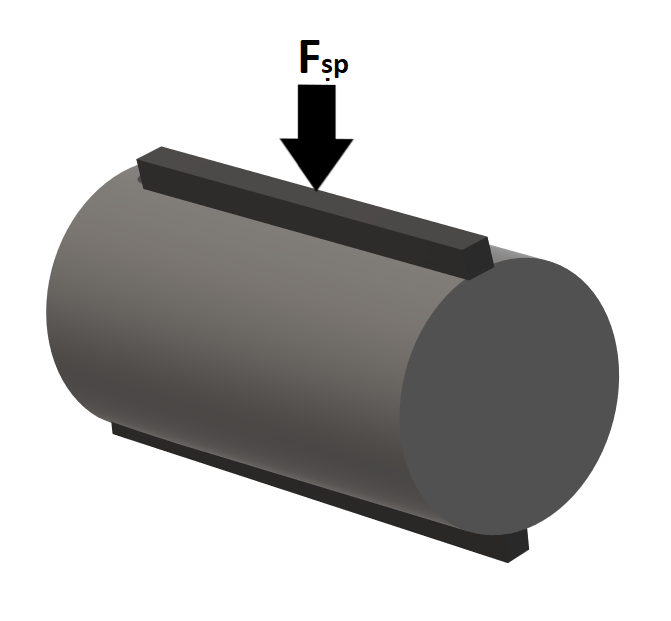
\includegraphics[width=6cm,height=5cm]{figures/Amir_Splitting_Theory.png}
\caption{The Brazilian disk test on a cylindrical sample with diameter and length of $D_{cyl}$ and $L_{cyl}$, respectively}
\label{fig:Amir_Splitting_Theory}
\end{figure} 

\begin{align}
\label{eq:Splitting_Strength}
\begin{split}
\sigma_{sp}=\frac{2f_{sp}}{\pi L_{cyl}D_{cyl}}
\end{split}
\end{align}

In the CAU Kiel laboratory, the splitting strength under THM processes is measured. To do so, a controlled temperature and humidity climate chamber (Fig. \ref{fig:Amir_Fracture_Toughness_Setup_b}) and a loading frame with a displacement transducer are required. Initially, the splitting test under room temperature condition with initial humidity of the sample is conducted. Afterwards, the temperature is raised to 50 and 80 $^{\circ}C$. The relative humidity can be controlled from 0 up to 100. Finally, the splitting strength, splitting Young’ modulus ($E_sp$) and load-displacement behavior are measured. The cylindrical claystone and saltstone samples are prepared in dimension of 100x200 $mm$ $(DxL)$ (Figure \ref{fig:Amir_Splitting_Sample}) and a strain rate of  0.1 \% is considered to insure a relatively fast loading rate. Fig. \ref{fig:Amir_Splitting_Setup} shows the placement of the sample under loading frame before performing the test.

\begin{figure}[!ht]
\centering
\begin{subfigure}[c]{0.3\textwidth}
\centering
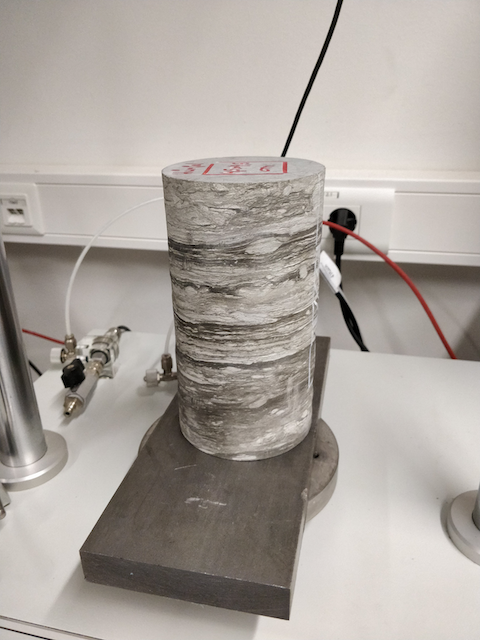
\includegraphics[width=4cm,height=5cm]{figures/Amir_Splitting_Sample.png}
\subcaption{}
\label{fig:Amir_Splitting_Sample}
\end{subfigure}
\hfill
\begin{subfigure}[c]{0.6\textwidth}
\centering
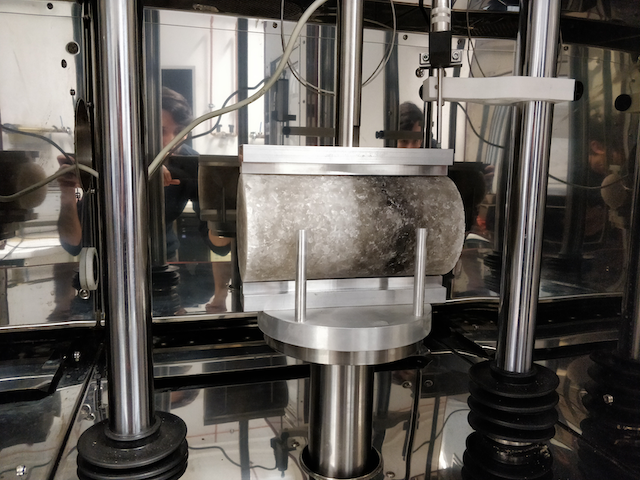
\includegraphics[width=6cm,height=5cm]{figures/Amir_Splitting_Setup.png}
\subcaption{}
\label{fig:Amir_Splitting_Setup}
\end{subfigure}
\caption{The sample preparation and test procedure (a) the claystone sample with a dimension of 100x200 $mm$, (b) the placement of saltstone inside of the climate chamber}
\end{figure}

Initially, the splitting strength of a saltstone samples under room temperature (20), 50 and 80 $^{\circ}C$ are measured. Due to a relatively homogeneous material property of the saltstone, the orientation of the sample will not affect the final outcomes. Figures \ref{fig:Amir_Splitting_Salt_20} and \ref{fig:Amir_Splitting_Salt_Result} depict the failure in 20 $^{\circ}C$ and load vs. displacement for different loading temperatures, respectively. The observed failure pattern for all of the setups is identical. The measured mean splitting strength using equation (\ref{eq:Splitting_Strength}) for 20, 50 and 80 $^{\circ}C$ are 1.65, 1.59 and 1.43 $MPa$, respectively. As a result, the temperature has a slight influence on the splitting strength of saltstone, especially when the temperature is raised up to 50 $^{\circ}C$.

\begin{figure}[!ht]
\centering
\begin{subfigure}[c]{0.35\textwidth}
\centering
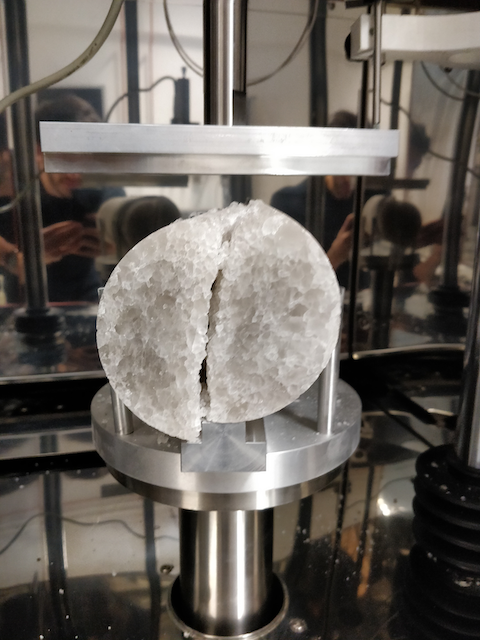
\includegraphics[width=4cm,height=5cm]{figures/Amir_Splitting_Salt_20.png}
\subcaption{}
\label{fig:Amir_Splitting_Salt_20}
\end{subfigure}
\hfill
\begin{subfigure}[c]{0.6\textwidth}
\centering
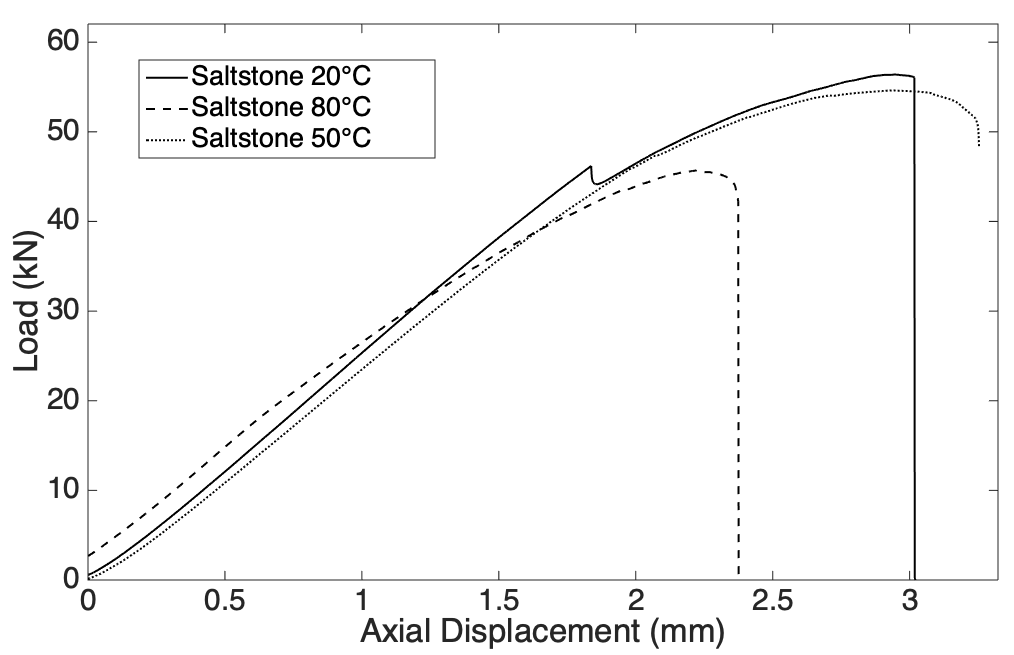
\includegraphics[width=6cm,height=5cm]{figures/Amir_Splitting_Salt_Result.png}
\subcaption{}
\label{fig:Amir_Splitting_Salt_Result}
\end{subfigure}
\caption{The splitting strength of a saltstone under different temperature conditions (a) the fracture path in saltstone in room temperature, (b) the load vs. displacement under different temperature conditions}
\end{figure}

The anisotropy of claystone and embedded layering orientation has a significant influence on material strength. To investigate the strength dependency on layering orientation, a series of tests, where the angle between the loading direction and layering orientation is 0 (parallel), 30, 45, and 90 (perpendicular) degree, is conducted. For 20 $^{\circ}C$, the failure pattern for 0, 45 and 90 degrees are provided in Figures \ref{fig:Amir_Splitting_Clay_0}, \ref{fig:Amir_Splitting_Clay_45} and \ref{fig:Amir_Splitting_Clay_90}. Fig. \ref{fig:Amir_Splitting_Clay_20_Result} depicts the load vs. displacement behavior of claystone with different layering degrees. 

\begin{figure}[ht!]
\centering
\begin{subfigure}[c]{0.48\textwidth}
\centering
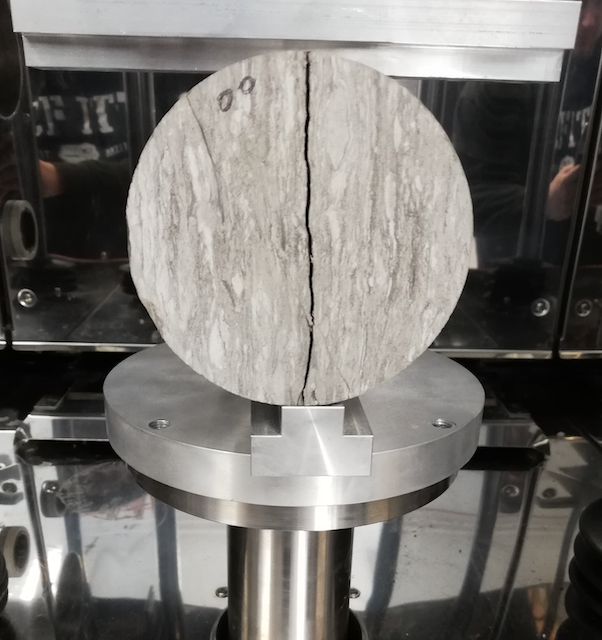
\includegraphics[width=5cm,height=5cm]{figures/Amir_Splitting_Clay_0.png}
\subcaption{}
\label{fig:Amir_Splitting_Clay_0}
\end{subfigure}
\hfill
\begin{subfigure}[c]{0.48\textwidth}
\centering
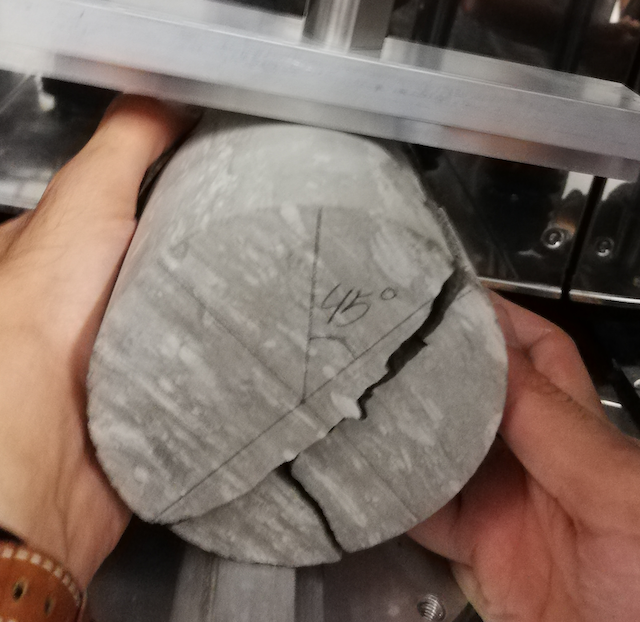
\includegraphics[width=5cm,height=5cm]{figures/Amir_Splitting_Clay_45.png}
\subcaption{}
\label{fig:Amir_Splitting_Clay_45}
\end{subfigure}
\hfill
\begin{subfigure}[c]{0.48\textwidth}
\centering
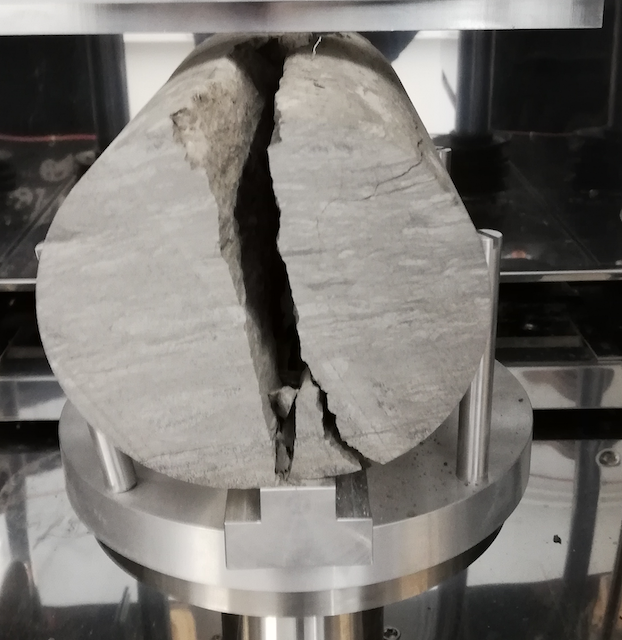
\includegraphics[width=5cm,height=5cm]{figures/Amir_Splitting_Clay_90.png}
\subcaption{}
\label{fig:Amir_Splitting_Clay_90}
\end{subfigure}
\caption{The fracture pattern under different layering orientation (a) 0 degrees, parallel, (b) 45 degrees, and (c) 90 degrees, perpendicular (20 $^{\circ}C$)}
\end{figure}

\begin{figure}[ht!]
\centering
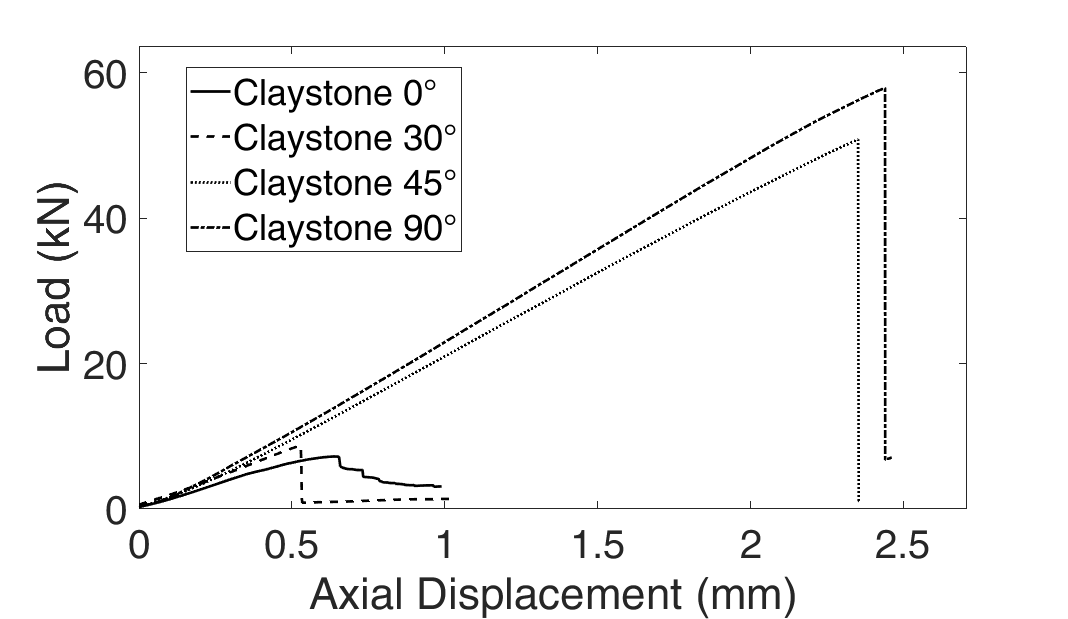
\includegraphics[width=9cm,height=5cm]{figures/Amir_Splitting_Clay_20_Result.png}
\caption{The load vs. displacement under different layering orientation, 20 $^{\circ}C$}
\label{fig:Amir_Splitting_Clay_20_Result}
\end{figure} 

Table \ref{table:Amir_Splitting_Table1} presents the mean outcome of the experimental tests for different orientation angles and temperature. The results depicts that when the loading is perpendicular to the layering orientation, the splitting strength of the claystone is almost 5 times higher than when it is parallel to the layering orientation. The temperature effect on splitting strength is negligible. 

\begin{table}[!ht]
\centering
\begin{center}
\begin{tabular}{ | >{\centering\arraybackslash}X m{8em} | >{\centering\arraybackslash}X m{3em}| >{\centering\arraybackslash}X m{3em} | >{\centering\arraybackslash}X m{3em} | >{\centering\arraybackslash}X m{3em} | >{\centering\arraybackslash}X m{3em} | }
\hline
Test Results & 0 $^{\circ}$ & 30 $^{\circ}$ & 45 $^{\circ}$ & 60 $^{\circ}$ & 90 $^{\circ}$ \\
\hline
$\sigma_{sp}$ ($MPa$) 20$^{\circ}C$ & 0.47 & 0.68 & 1.13 & 1.45 & 1.92  \\ 
\hline
$\sigma_{sp}$ ($MPa$) 80$^{\circ}C$ & 0.52 & 0.64 & 1.02 & 1.25 & 1.86   \\
\hline
\end{tabular}
\end{center}
\caption{The splitting tensile strength of the Opalinus claystone with different temperature and layering orientations}
\label{table:Amir_Splitting_Table1}
\end{table}
